% Chapter 2: Background

\chapter{Background} % Chapter title
\addtocontents{lof}{\protect\vspace{\beforebibskip}}%

\label{chapter:background}
\label{chapter:state-of-the-art}

\lettrine[lines=3, loversize=0.1]{I}{n this chapter} we will introduce and discuss the technical background of this thesis.
We will start by discussing the structure and functionality of multi-core \CPUs and \GPUs.
We will focus on \GPUs as their architecture is quite different to traditional \CPUs, and because \GPUs will be the main hardware target of our \SkelCL programming model presented later.
Then we will discuss the most common programming approaches for multi-core \CPUs and \GPUs, with a particular focus on \OpenCL.

We will then introduce the idea of structured parallel programming and discuss its origin in functional programming.
In this approach, predefined parallel patterns (\aka, \emph{algorithmic skeletons}) hiding the complexities of parallelism are used for expressing parallel programs.
This thesis builds upon this idea, developing a structured parallel programming model for \GPUs and a novel compilation technique that transforms pattern-based programs to efficient hardware-specific implementations.
% We will finish this chapter by discussing several state-of-the-art implementations of structured parallel programming for cluster systems and multi-core \CPUs.

\section{Modern Parallel Processors}
% structure and functionality of:
As discussed in the introduction in \autoref{ch:introduction}, virtually all modern processors feature multiple cores to increase their performance and energy efficiency.
Here we will look at two major types of modern parallel processors: multi-core \CPUs and \GPUs.
Multi-core \CPUs are \emph{latency-oriented} architectures~\cite{GarlandK10}, \ie, they are optimized to hide memory latencies with large caches and various other advanced architectural features, like out-of-order execution and extensive branch prediction.
\GPUs are \emph{throughput-oriented} architectures~\cite{GarlandK10}, \ie, they are optimized to increase the overall computational throughput of many parallel tasks instead of optimizing single task performance.

We will discuss both architectures in the following two sections.

\subsection{Multi-Core \CPUs}
% multi-core CPUs
\autoref{fig:multicore} shows an abstract representation of a typical multi-core \CPU architecture, like Intel's latest \CPU architecture: Haswell~\cite{IntelHaswell}.
\begin{figure}
  \centering
  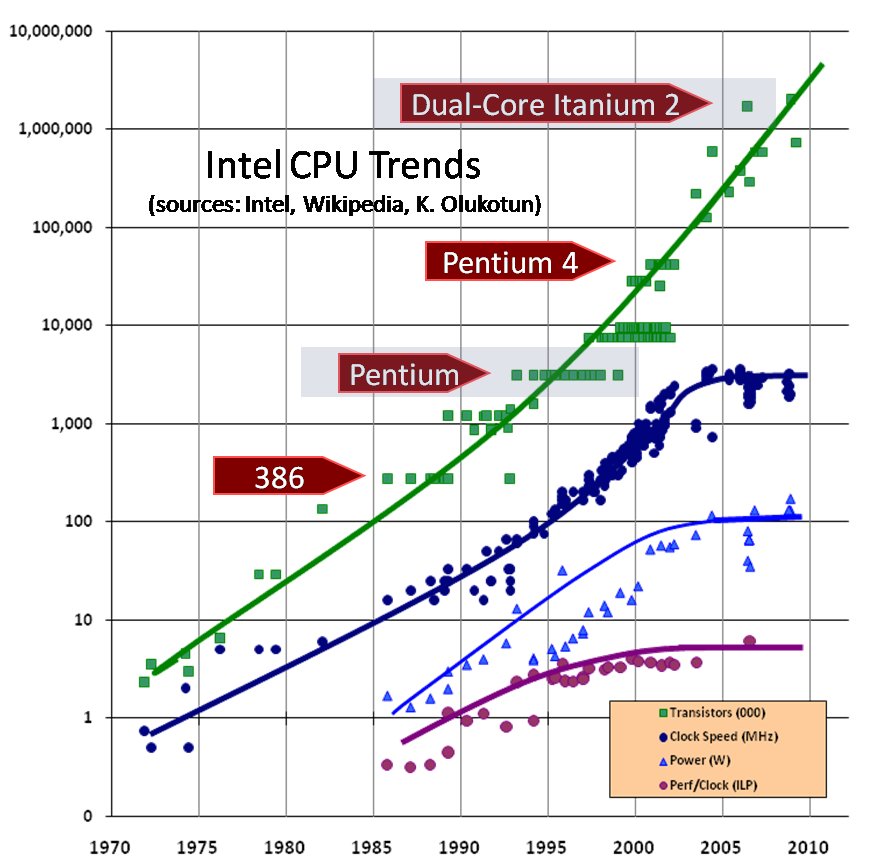
\includegraphics[width=.75\textwidth]{CPU}
  \caption{Overview of a multi-core \CPU architecture}
  \label{fig:multicore}
\end{figure}
% describe caches
The \CPU is divided into multiple cores each of which features two levels of caches.
The smallest but fastest cache is called L1 cache and is typically divided into a distinct cache for instructions and a data cache, each of 32 kilobyte for the Haswell architecture.
Each core also features a second level cache (L2 cache) of 256 kilobyte for the Haswell architecture.
The \CPU has a large cache (L3 cache) which is shared by all cores.
This cache is often several megabytes large, for Intel's Haswell architecture the L3 cache is at least 2 and up to 45 megabytes in size.

% describe core: branch prediction, out-of-order execution, SIMD units
Each \CPU core performs computations completely independently of the other cores, and it consists itself of multiple execution units which can perform computations in parallel.
This happens transparently to the programmer even when executing a sequential program.
The \CPU core exploits \emph{instruction level parallelism} (ILP) by performing out-of-order execution which re-orders instructions prior to execution while still respecting their dependencies:
\eg, if two or more instructions have no dependencies then they can be executed in parallel.
In the Intel Haswell architecture, 4 arithmetic operations and 4 memory operations can be performed in parallel in one clock cycle on every core.
Furthermore, most modern \CPU architectures support SIMD vector extensions like the \emph{Advanced Vector Extensions} (AVX) or the older \emph{Streaming SIMD Extensions} (SSE).
These extensions add additional instructions to the instruction set architecture, allowing the compiler to generate code explicitly grouping data into vectors of small fixed sizes which can be processed in parallel.
The current AVX extension allows vectors of up to 256 bits, \eg, a grouping of 8 single precision floating point numbers, to be processed in parallel.
Most modern optimizing compilers perform some form of automatic vectorization, but often programmers vectorize programs manually when the compiler fails to generate sufficiently optimized code.

% make conclusions: latency oriented => caches important, good performance for single and multiple threads, comparably low core count and hyper threading -> limited thread-level parallelism
The design of multi-core \CPUs is motivated by the overall goal to provide high performance when executing multi-threaded programs and still have a high single-core performance when executing sequential programs~\cite{GarlandK10}.
This is why the individual cores have a quite sophisticated design to achieve executing a series of instructions as fast as possible, by applying out-of-order execution and exploiting architectural features like a deep pipeline for decoding and executing instructions combined with advanced branch prediction.
Unfortunately, the design of these complex cores makes switching between the threads running on the same core relatively expensive, as the execution pipeline has to be flushed and the register content for the first thread has to be saved before resuming the execution on the second thread.
To address this issue, some multi-core architectures feature \emph{Simultaneous Multi-Threading} (SMT), \aka, \emph{hyper threading}:
a single \CPU core can execute multiple (usually 2 or 4) threads in parallel and switching between the threads is cheap.
This technique is used to mitigate the effect which memory latency can have on the execution:
if a thread is waiting for a memory request then another thread can continue executing.
The other central component used to prevent waiting times for memory requests is the cache hierarchy.
As we will see, multi-core \CPUs feature considerably larger caches than \GPUs.
The caches help to keep the threads running in parallel on the multi-core \CPU busy.

% Possible optimizations
Among the most important optimizations to achieve high performance on modern multi-core \CPUs are:
exploiting the SIMD vector extensions and optimizing the cache usage~\cite{IntelCPUOptimizingGuide}.

\subsection[Graphics Processing Units (GPUs)]{Graphics Processing Units}
  % GPUs
\autoref{fig:gpu} shows an abstract representation of a typical \GPU architecture, like Nvidia's latest high-performance computing \GPU architecture: Kepler~\cite{CUDAKepler2012}.
\begin{figure}
  \centering
  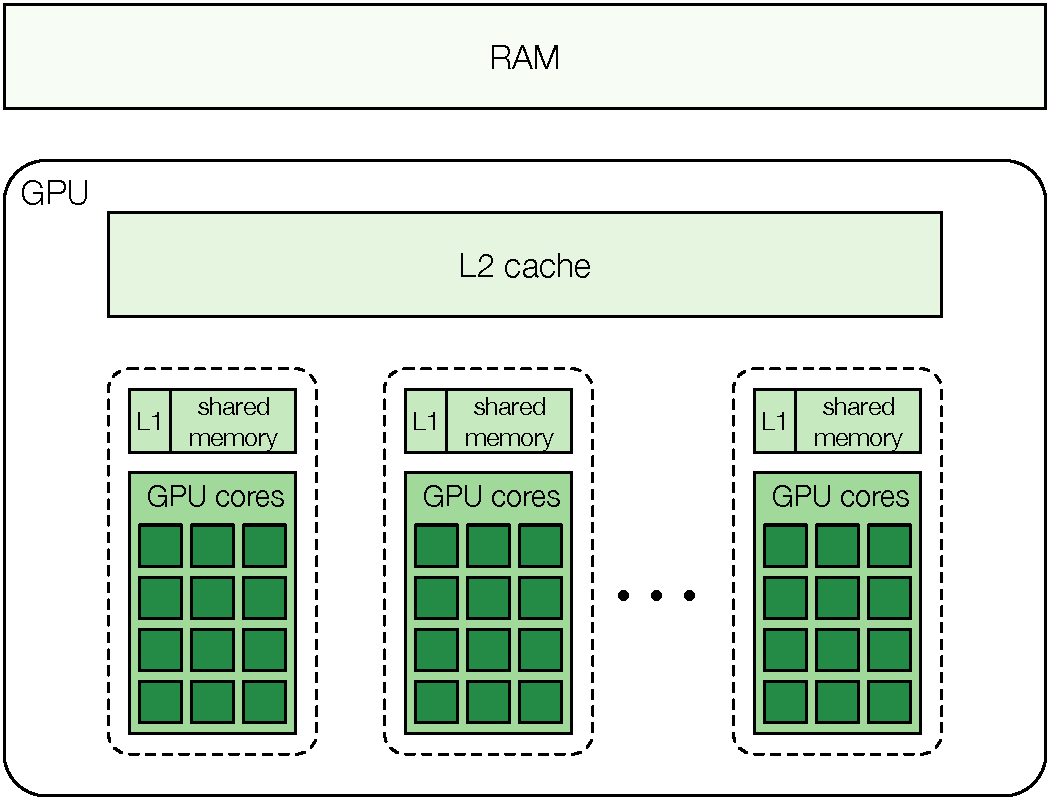
\includegraphics[width=.75\textwidth]{GPU}
  \caption{Overview of a \GPU architecture}
  \label{fig:gpu}
\end{figure}
% describe cores and execution
While the overall design looks fairly similar to the design of the multi-core \CPU, the architecture of the \GPU is actually very different in its details.
The lightweight \GPU cores are grouped together into what Nvidia calls a \emph{Streaming Multiprocessor} (SM).
In the Kepler architecture, an SM features 192 single-precision cores, 64 double-precision units, 32 special function units, and 32 memory units.
% \autoref{fig:gpuSM} shows the design of an SM in the Kepler architecture.
The 192 single-precision cores are very lightweight compared to the complex \CPU cores we discussed in the previous subsection.
A single \GPU core does not support SIMD vectorization:
it performs the straightforward in-order execution, and does not perform complex branch prediction.
This design makes the implementation of such a core in hardware cheap and enables the grouping of hundreds of cores in a single SM.

% describe caches and memory
Modern \GPUs feature two levels of caches:
the first level (L1) is private to each SM and the second level cache (L2) is shared among all SMs.
Compared to the cache sizes of the \CPU, the caches on the \GPU are fairly small.
The Kepler architecture features an L1 cache of 48 kilobyte and an L2 cache of 1.5 megabyte.
It is important to notice that these caches are shared by a vast amount of threads being executed on the \GPU:
the 48 kilobyte L1 caches are shared among up to 2048 threads being executed on a particular SM and the L2 cache is shared among up to about 30,\,000 threads.

Besides caches, each SM on a \GPU features also a scratchpad memory, called \emph{shared memory} in Nvidia's \GPU architectures.
This memory is small (16 or 48 kilobytes) but very fast (comparably to the L1 cache).
While the L1 cache is automatically managed by a cache controller, the shared memory is explicitly managed by the programmer.

% make conclusions: throughput oriented => cores and threads important, different trade off: poor performance for single thread very good performance for data parallel applications => bad when: a lot of branching, less caches => memory accesses are expensive (coalescing ...)
The design of \GPUs is motivated by the overall goal to deliver maximal throughput even if this requires to sacrifice the performance of single threads~\cite{GarlandK10}.
This is why the \GPU cores are lightweight offering poor sequential performance, but thousands of cores combined together offer a very high computational throughput.
Memory latencies are mitigated by a high oversubscription of threads:
in the Kepler architecture an SM can manage up to 2048 threads which can be scheduled for execution on the 192 cores.
If a thread is waiting for a memory request, another thread continues its execution.
This is the reason why caches are fairly small, as they play a less important role as in \CPU architectures.

\paragraph{GPU Thread Execution}
The execution of threads on a \GPU is very different as compared to the execution on a traditional multi-core \CPU:
multiple threads are grouped by the hardware and executed together.
Such a group of threads is called a \emph{warp} by Nvidia.
In the Kepler architecture, 32 threads form a warp and an SM selects 4 warps and for each warp 2 independent instructions are selected to be executed in parallel on its single-precision cores, double-precision units, special function units, and memory units.

All threads grouped into a warp perform the same instructions in a lockstep manner.
Is is possible that two or more threads follow different execution paths.
In this case, all threads sharing a common execution path execute together while the other threads pause their execution.
It is beneficial to avoid warps with divergent execution paths, as this reduces or eliminates the amount of threads pausing their execution.
Nvidia calls this execution model: \emph{single-instruction, multiple-thread} (SIMT).

Programmers are advised to manually optimize their code, so that all threads in a warp follow the same execution path.
Threads in the same warp taking different branches in the code can substantially hurt the performance and should, therefore, be avoided.

\paragraph{GPU Memory Accesses}
Accessing the main memory of a \GPU, called \emph{global memory}, is an expensive operation.
The \GPU can optimize accesses when the global memory is accessed in certain fixed patterns.
If the threads organized in a warp access a contiguous area of the memory, the hardware can \emph{coalesce} the memory access, \ie, perform a single memory request instead of issuing individual requests for every thread.
Several similar access patterns exist which are detected by the hardware to coalesce the memory accesses by multiple threads.

This is a major optimization opportunity for many \GPU programs, as the available memory bandwidth can only be utilized properly if memory accesses are coalesced.
Uncoalesced memory accesses may severely hurt the performance.


\paragraph{GPU Shared Memory}
% shared memory
The usage of the shared memory featured in each SM can substantially increase performance -- when used properly.
The programmer is responsible for exploiting this memory by explicitly moving data between the global memory and the shared memory.
All threads executing on the same SM have shared access to the shared memory at a high bandwidth and with low latency.
When multiple threads need to access the same data item, it is often beneficial to first load the data item into the shared memory by a single thread and perform all successive accesses on the shared memory.
This is similar to a cache with the difference that the programmer has to explicitly control its behavior.
Shared memory can also be used by a thread to efficiently synchronize and communicate with other threads running on the same SM.
On current \GPUs, global synchronization between threads running on different SMs is not possible.
% it is only possible for threads running on the same SM to synchronize, because global synchronization between threads running on different SMs is not possible.

\bigskip
Summarizing, current \GPU architectures are more sensitive to optimizations than \CPU architectures.
The most important optimizations on \GPUs are:
exploit the available parallelism by launching the right amount of threads, ensure that accesses to the global memory are coalesced, use the shared memory to minimize accesses to the global memory, and avoid divergent branches for threads organized in a warp~\cite{CUDATuningKepler2015}.

\noindent
In addition to these optimizations, it is important for the programmer to keep in mind that the application exploiting the \GPU is still executed on the \CPU and typically only offloads computation-intensive tasks to the \GPU.
An often crucial optimization is to minimize the data transfer between the \CPU and the \GPU or overlap this transfer with computations on the \GPU.

\bigskip

\noindent
We now discuss the current approaches to program multi-core \CPUs and \GPUs in detail.



\section{Programming of Multi-Core CPUs and GPUs}
Arguably the most popular programming approach for multi-core \CPUs is \emph{multithreading}.
Threading libraries exist for almost all popular programming languages, including C~\cite{Cstandard,Pthreads} and \Cpp~\cite{Cppstandard}.
Threads are conceptionally similar to processes in an operating system, with the major difference that threads share the same address space in memory while processes usually do not.
This enables threads to communicate and cooperate efficiently with each other by directly using the same memory.
Programmers have great flexibility and control over the exact behavior of the threads and their interaction, including the important questions of when and how many threads to use, how tasks and data are divided across threads, and how threads synchronize and communicate with each other.
The disadvantage of this high flexibility is that the burden of developing a correct and efficient program lies almost entirely on the programmer.
The interaction of threads executing concurrently can be very complex to understand and reason about, and traditional debugging techniques are often not sufficient as the execution is not deterministic any more.

\OpenMP~\cite{OpenMP} is a popular alternative approach focusing on exploiting parallelism of loops in sequential programs.
The focus on loops is based on the observation that loops often iterate over large data sets performing operations on every data item without any dependencies between iterations.
Such workloads are traditionally called \emph{embarrassingly parallel} and can be parallelized in a straightforward manner.
In \OpenMP, the programmer annotates such loops with compiler directives, and a compiler supporting the \OpenMP standard automatically generates code for performing the computations of the loop in parallel.
Recent versions of the \OpenMP standard and the closely related \OpenACC~\cite{OpenACC} standard support execution on \GPUs as well.
Here the programmer has to additionally specify the data regions which should be copied to and from the \GPU prior to and after the computation.
\OpenMP and \OpenACC allow for a fairly easy transition from sequential code to parallel code exploiting multi-core \CPUs and \GPUs.
Performance is often not optimal as current compilers are not powerful enough to apply important optimizations like cache optimizations, ensuring coalesced memory accesses, and the usage of the local memory.

\CUDA~\cite{CUDAProgrammingGuide} and \OpenCL~\cite{OpenCL} are the most popular approaches to program \GPU systems.
While \CUDA can only be used for programming \GPUs manufactured by Nvidia, \OpenCL is a standard for programming \GPUs, multi-core \CPUs, and other types of parallel processors regardless of their hardware vendor.
All major processor manufactures support the \OpenCL standard, including AMD, ARM, IBM, Intel, and Nvidia.
We will study the \OpenCL programming approach in more detail, as it is the technical foundation of the work presented later in \autoref{part:skelcl} and \autoref{part:codeGeneration} of this thesis.


\subsection{The OpenCL Programming Approach}
\OpenCL is a standard for programming multi-core \CPUs, \GPUs, and other types of parallel processors.
\OpenCL was created in 2008 and has since been refined multiple times.
In this thesis, we will use the \OpenCL standard version 1.1 which was ratified in June 2010.
This is the most commonly supported version of the standard with support from all major hardware vendors: AMD, ARM, Intel, and Nvidia.
The newer \OpenCL standards version 2.0 and 2.1 are currently not supported on Nvidia \GPUs.

\OpenCL is defined in terms of four theoretical models: platform model, memory model, execution model, and programming model.
We will briefly discuss all four models.

\paragraph{The \OpenCL Platform Model}
\autoref{fig:opencl} shows the \OpenCL platform model.
\OpenCL distinguishes between a \emph{host} and multiple \OpenCL \emph{devices} to which the host is connected.
In a system comprising of a multi-core \CPU and a \GPU, the \GPU constitutes an \OpenCL device and the multi-core \CPU plays the dual rule of the host and an \OpenCL device as well.
An \OpenCL application executes sequentially on the host and offloads parallel computations to the \OpenCL devices.

\OpenCL specifies that each device is divided into one or more \emph{compute units} (CU) which are again divided into one or more \emph{processing elements} (PE).
When we compare this to our discussion of multi-core \CPUs, there is a clear relationship:
a \CPU core corresponds to a compute unit and the functional units inside of the \CPU core performing the computations correspond to the processing elements.
For the \GPU the relationship is as follows:
a streaming multiprocessor corresponds to a compute unit and the lightweight \GPU cores correspond to the processing elements.

\begin{figure}
  \centering
  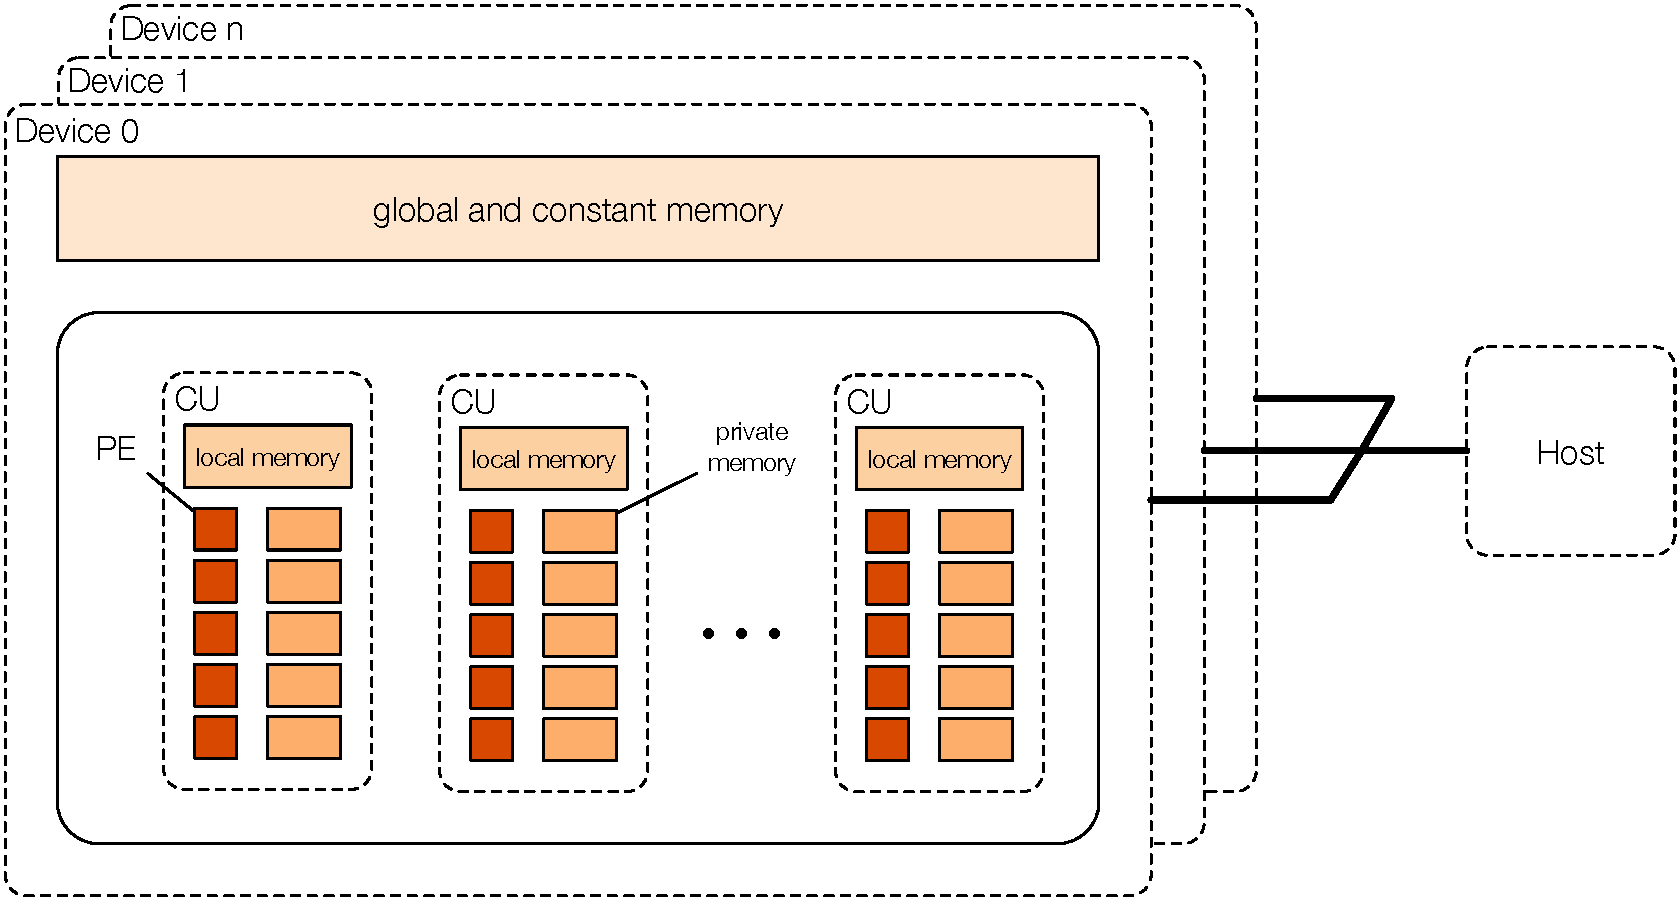
\includegraphics[width=.95\textwidth]{OpenCL}
  \caption{The \OpenCL platform and memory model}
  \label{fig:opencl}
\end{figure}

\paragraph{The \OpenCL Memory Model}
Each device in \OpenCL has its own memory.
This memory is logically (but not necessarily physically) distinct from the memory on the host.
Data has to be moved explicitly between the host and device memory.
The programmer issues commands for copying data from the host to the device and vice versa.

On a device, \OpenCL distinguishes four memory regions:
global memory, constant memory, local memory, and private memory.
These memory regions are shown in \autoref{fig:opencl}.

The \emph{global memory} is shared by all compute units of the device and permits read and write modifications from the host and device.
% Dynamic memory allocations are possible from the host, but there is no possibility to allocate global memory from the device side.
The global memory is usually the biggest but slowest memory area on an \OpenCL device.

The \emph{constant memory} is a region of the global memory which remains constant during device execution.
% The host can dynamically allocate regions of the constant memory and can read and write to it.
% The device can statically allocate constant memory and only read from it.
The host can read and write to the constant memory, but the device can only read from it.

The \emph{local memory} is a memory region private to a compute unit.
It permits read and write accesses from the device; the host has no access to tis memory region.
% Memory can either be allocated dynamically from the host or statically from the device.
The local memory directly corresponds to the fast per-SM shared memory of modern \GPUs.
On multi-core \CPUs, the local memory is usually only a logical distinction:
local memory is mapped to the same physical memory as the global memory.

The \emph{private memory} is a memory region private to a processing element.
The device has full read and write access to it, but the host has no access at all.
The private memory contains all variables which are private to a single thread.


\paragraph{The \OpenCL Execution Model}
The communication between the host and a particular device is performed using a \emph{command queue}.
The host submits commands into a \emph{command queue} which by-default processes all commands in the first-in-first-out order.
It is also possible to configure command queues to operate out-of-order, \ie, no order of execution of commands is guaranteed.

There exist three types of commands which can be enqueued in a command queue.
A \emph{memory command} indicates to copy data from the host to the device or from the device to the host.
A \emph{synchronization command} enforces a certain order of execution of commands.
Finally, a \emph{kernel execution command} executes a computation on the device.

A \emph{kernel} is a function which is executed in parallel on an \OpenCL device.
\autoref{lst:openclExample} shows a simple \OpenCL kernel performing matrix multiplication.
When launching a kernel on a device, the programmer explicitly specifies how many threads will execute in parallel on the device.
A thread executing a kernel is called a \emph{work-item} in \OpenCL.
Work-items are grouped together in \emph{work-groups} which allow a more coarse-grained organization of the execution.
All work-items of a work-group share the same local memory, and synchronization between work-items of the same work-group is possible but it is forbidden for work-items from different work-groups.
This is because all work-items from the same work-group are guaranteed to be executed on the same CU, but this guarantee does not hold for work-items from different work-groups.

\begin{lstlisting}[float, caption={Example of an \OpenCL kernel.}, label={lst:openclExample}]
kernel void matMultKernel(global float* a, global float* b,$\label{lst:openclExample:1}$
                          global float* c, int width) {$\label{lst:openclExample:2}$
 int colId = get_global_id(0); int rowId = get_global_id(1);$\label{lst:openclExample:3}$

 float sum = 0.0f;
 for (int i = 0; i < width; ++i)
   sum += a[rowId * width + k] * b[k * width + colId];

 c[rowId * width + colId] = sum;
}
\end{lstlisting}

\OpenCL kernels are implemented in a dialect of C (starting with \OpenCL 2.1 a dialect of \Cpp) with certain restrictions as well as extensions.
The most prominent restrictions are:
recursive functions and function pointers are not supported, as well as system calls, including \code{malloc}, \code{printf}, file I/O, etc.
The most important extensions are:
qualifiers for pointers reflecting the four address spaces (\eg, the \code{global} qualifier in \autoref{lst:openclExample:1} and \autoref{lst:openclExample:2} of \autoref{lst:openclExample}) and vector data types, like \code{float4}.
Moreover, \OpenCL provides a set of functions which can be used to identify the executing work-item and work-group.
One example is the \code{get\_global\_id} function used in \autoref{lst:openclExample:3} of \autoref{lst:openclExample}.
This is usually used so that different work-items operate on different sets of the input data.
In \autoref{lst:openclExample}, each work-item computes one item of the result matrix \code{c} by multiplying and summing up a row and column of the input matrices \code{a} and \code{b}.
This kernel only produces the correct result if exactly one work-item per element of the result matrix is launched.
If the host program launches a different configuration of work-items then only part of the computation will be performed or out-of-bound memory accesses will occur.

\paragraph{The \OpenCL Programming Model}

\OpenCL supports two programming models: data parallel programming and task parallel programming.
The predominant programming model for \OpenCL is the data parallel programming model.

In the \emph{data parallel programming model}, kernel are executed by many work-items organized in multiple work-groups.
Parallelism is mainly exploited by the work-items executing a single kernel in parallel.
This programming model is well suited for exploiting modern \GPUs and, therefore, widely used.
This model is also well suited for modern multi-core \CPUs.

In the \emph{task parallel programming model}, kernels are executed by a single work-item.
Programmers exploit parallelism by launching multiple tasks which are possibly executed concurrently on an \OpenCL device.
This programming model is not well suited for exploiting the capabilities of modern \GPUs and, therefore, not widely used.

\section{Structured Parallel Programming}
% structured parallel programming & functional foundations
\emph{Structured programming} emerged in the 1960s and 1970s as a reaction to the ``software crises''.
Back then (and still today) programs were often poorly designed, hard to maintain, and complicated to reason about.
Dijkstra identified the low-level \code{goto} statement as a major reason for programmers writing ``spaghetti code''.
In his famous letter~\cite{Dijkstra68a}, he argued that programs should organize code more structurally in procedures and using higher-level control structures like \code{if} and \code{while}.
Dijkstra's letter helped to eventually overcome unstructured sequentiell programming and to establish structured programming~\cite{DahlDiHo1972}.
The new structures proposed to replace \code{goto} where suggested based on observations of common use cases -- or \emph{patterns} of use -- of the \code{goto} statement in sequential programming.
By capturing an entire pattern of usage, these patterns raise the abstraction level and make it easier to reason about them.
An \code{if A then B else C} statement has a clear semantic which is easy to understand and reason about, for example is it clear to the programmer -- and the compiler -- that \code{B} and \code{C} cannot both be executed.
This helps the programmer to understand the source code and the compiler to produce an optimized executable.
The equivalent unstructured code containing multiple \code{goto} statements obtains the same high-level semantic by combining the low-level operations with their low-level semantics.
Both, programmer and compiler, have to ``figure out'' the high-level semantic by means of analyzing the sequence of low-level operations and reconstructing the overall semantic.

In recent years researchers have suggested similar arguments to Dijkstra's for addressing the challenges attached with traditional parallel programming by introducing \emph{structured parallel programing}.
For parallel programming using message passing, Gorlatch argues similar to Dijkstra that single send and receive statements should be avoided and replaced by collective operations~\cite{Gorlatch04}.
Each collective operation, \eg, broadcast, scatter, or reduce, captures a certain common communication pattern traditionally implemented with individual send and receive statements.
In~\cite{McCoolRoRe2012}, the authors argue that \emph{structured parallel patterns}, each capturing a common computation and communication behavior, should be used to replace explicit thread programming to improve the maintainability of software.
The book discusses a set of parallel patterns and their implementation in different recent programming approaches.
The underlying ideas go far back to the 1980s when Cole was the first to introduced \emph{algorithmic skeletons} to structure and, therefore, simplify parallel programs~\cite{Cole1991}.
As with sequential structured programming, structured parallel programming raises the abstraction level by providing high-level constructs: collective operations, parallel patterns, or algorithmic skeletons.
The higher level of abstraction both simplifies the reasoning about the code for the programmer and enables higher-level compiler optimizations.

As our work directly extends the ideas of Cole, we will discuss algorithmic skeletons in more detail next.

\subsection{Algorithmic Skeletons}
Cole introduced algorithmic skeletons as special higher-order functions which describe the ``computational skeleton'' of a parallel algorithm.
Higher-order functions are a well-known concept in functional programming and describe functions accepting other functions as arguments or returning a function as result.
This is often useful, as it allows to write more abstract and generic functions.

An example for an algorithmic skeletons is the \emph{divide \& conquer skeleton} which was among the original suggested skeletons by Cole~\cite{Cole1991}:
\begin{align*}
  D_C\ indivisible\ split\ join\ f% &= F\\
%  \textit{where}\ F\ P &= f\ P, \textit{ if  } indivisible\ P\nonumber\\
%                     &= join\ (map\ F\ (split\ P)), \textit{ otherwise}\nonumber
\end{align*}
The algorithmic skeleton $D_C$ accepts four functions as its arguments:
\begin{itemize}
  \item $indivisible$ is a function deciding if the given problem should be decomposed (divided) or not,
  \item $split$ is a function decomposing a given problem into multiple sub-problems,
  \item $join$ is a function combining multiple solved sub-problems into a larger solution,
  \item $f$ is a function solving an indivisible problem, \ie, the base case.
\end{itemize}

Applications like the discrete Fourier transformation, approximate integration, or matrix multiplication can be expressed and implemented using this algorithmic skeleton.
The application developer provides implementations for the functions required by the algorithmic skeleton to obtain a program which can be applied to the input data.

An algorithmic skeleton has a parallel implementation.
In the example of the $D_C$ skeleton, the implementation follows the well-known divide \& conquer technique which divides problems into multiple sub-problems which can be solved independently in parallel.
The implementation of the algorithmic skeleton hides the complexities of parallelism from the user.
It, therefore, provides a higher-level interface abstracting away the details of the parallel execution, including low-level details like launching multiple threads, as well as synchronization and communication of threads.

\paragraph{A Classification of Algorithmic Skeletons}
Algorithmic skeletons can broadly be classified into three distinct classes~\cite{Gonzalez-VelezL10}:
\begin{itemize}
  \item \emph{data-parallel skeletons} transform typically large amounts of data,
  \item \emph{task-parallel skeletons} operate on distinct tasks which potentially interact with each other,
  \item \emph{resolution skeletons} capture a family of related problems.
\end{itemize}

Examples of data-parallel skeletons are \emph{map} which applies a given function to each element of its input data in parallel, or \emph{reduce} which performs a parallel reduction based on a given binary operator.
Well known task-parallel skeletons are \emph{farm (\aka, master-worker)} where independent tasks are scheduled for parallel execution by the workers, or \emph{pipeline} where multiple stages are connected sequentially and the execution of all stages can overlap to exploit parallelism.
Finally, the discussed $D_C$ skeleton is an example of a resolution skeleton which captures the family of problems which can be solved by applying the divide \& conquer technique.

In this thesis, we will mainly focus on data-parallel skeletons, as they are especially suitable for the data-parallel \GPU architecture.
We will also introduce two new resolution skeletons which capture two specific application domains for which we can provide efficient \GPU implementations as well.

\subsection{Advantages of Structured Parallel Programming}
Structured parallel programming offers various advantages over the traditional unstructured parallel programming.

\bigskip

\paragraph{Simplicity}
Structured parallel programming raises the level of abstraction by providing higher-level constructs which serve as basic building blocks for the programmer.
Lower-level details are hidden from the programmer and handled internally by the implementation of the algorithmic skeletons.
This simplifies the reasoning about programs and helps in the development process, as well as increases the maintainability of the software.

\paragraph{Safety and Determinism}
Potentially dangerous low-level operations are not used directly by the programmer in structured parallel programming.
Therefore, issues like deadlocks and race conditions can be entirely avoided -- given a correct and safe implementation of the provided algorithmic skeletons.
Furthermore, the high-level semantic of the algorithmic skeletons can guarantee determinism, while the lacking of determinism due to the parallel execution is a major concern in low-level, unstructured parallel programming; this concern complicates development and debugging of the software.

\paragraph{Portability}
% portability of functionality
Algorithmic skeletons offer a single high-level interface but can be implemented in various ways on different hardware systems.
Existing skeleton libraries target distributed systems~\cite{Kuchen02,AldinucciCDKT12,MatsuzakiKIHA04}, shared memory systems like multi-core \CPUs~\cite{AldinucciDaKiTo2011,CiechanowiczK10,LeytonP10}, and -- as we will discuss in this thesis -- systems with multiple \GPUs as well.
In contrary, unstructured parallel programming commits to a low-level programming approach targeting a particular hardware architecture, thus, making portability a major issue.
Furthermore, algorithmic skeletons evolved from functional programming and are, therefore, by-nature composabel and offer a high degree of re-use.

% performance portability
Another issue of portability is the portability of performance:
can a certain level of performance be obtained when switching from one hardware architecture to another?
This is virtually absent from low-level unstructured parallel programming as programmers apply low-level hardware-specific optimizations to achieve high performance.
These optimizations are usually not portable, as we will show later in \autoref{chapter:codeGeneration}.
Performance portability is a challenging and timely research topic which we address in this thesis by introducing a novel approach using structured parallel programming to achieve performance portability.

\pagebreak
\paragraph{Predictability}
The structure and regularity of structured parallel programming allows to build performance models which can be used in the development process to estimate the performance of the developed software.
Many research projects are devoted to this topic, showing that it is possible to predict the runtime of programs expressed with algorithmic skeletons~\cite{HayashiC02,DarlingtonFHKSW93,BischofGK03,Alt2007,StegmeierFrJAUn2015}.
Examples for related work in this area include work on particular algorithmic skeletons~\cite{BischofGK03}, work targeted towards distributed and grid systems~\cite{Alt2007}, and recently work targeting real-time systems~\cite{StegmeierFrJAUn2015}.

\paragraph{Performance and Optimizations}
Many studies have shown that structured parallel programs can offer the same level of performance as programs implemented and optimized with traditional unstructured techniques.
Examples include application studies on grid systems~\cite{Alt2007}, distributed systems~\cite{CiechanowiczKSGK09}, as well as systems featuring multi-core \CPUs~\cite{AldinucciMT10}.
In this thesis, we will investigate the performance of programs expressed with data-parallel algorithmic skeletons on systems with one or multiple \GPUs.

The high-level semantic of algorithmic skeletons enable high-level optimizations like the rewrite rules presented in~\cite{Gorlatch00}.
These optimizations exploit information about the algorithmic structure of a program which is often hard or impossible to extract from unstructured programs.
In this thesis, we will present a system for encoding and systematically applying such high-level optimizations to generate highly optimized code from a high-level, skeleton-based program representation.


%\from{HIPS begin}
%\section{GPU programming using OpenCL (HIPS)}
%
%The OpenCL standard~\cite{OpenCL} can be used for programming any OpenCL-capable device.
%These devices embrace most modern GPUs and other accelerators, e.\,g., the Cell BE, as well as standard multi-core CPUs.
%
%OpenCL distinguishes between a \emph{host} system, usually containing one or several CPUs, and \emph{devices} that are integrated into the host system.
%An OpenCL device logically consists of one or more \emph{compute units} (CUs) that are divided into one or more \emph{processing elements} (PEs).
%All computation on the device is performed in the PEs.
%OpenCL applications run on the host and call \emph{kernel functions} which are executed simultaneously by multiple PEs on one or more devices.
%A single instance of a kernel function is called a \emph{work-item} and can be identified by its \emph{global ID}.
%Every work-item executes the same code, but the execution can vary per work-item due to branching according to the global ID.
%Work-items are organized in \emph{work-groups}.
%When a kernel function is started, the host code specifies how many work-items are launched and how many work-items form a work-group.
%All work-items in one work-group are executed on the same CU.
%Therefore, the size of a work-group can have a significant effect on the runtime performance.
%
%In OpenCL, host and device have separate memories.
%Thus, functions are provided to transfer data from the host's to the device's memory (\emph{upload}) and back (\emph{download}).
%Memory areas have to be allocated on the device before data can be accessed by it and deallocated thereafter.
%
%For portability across a wide range of devices, kernel functions are compiled at runtime.
%The host program passes the kernel's source code as a plain string to the OpenCL driver to create executable binary code.
%This is different compared to CUDA which provides a special compiler \texttt{nvcc} to compile the device code and the host code.
%
%Creating applications for multi-GPU systems introduces new challenges, like partitioning the application appropriately and, explicitly implementing data transfer between devices~\cite{SchellmannVG08}.
%The host application must coordinate and perform synchronization and data exchange explicitly.
%The source code for performing such exchanges further increases the amount of boilerplate code.
%
%In the following, we describe how our SkelCL library addresses these problems of GPGPU programming.
%\from{HIPS end}
%
%
%\from{HiStencils begin}
%\section{Stencils Using OpenCL (HiStencils)}
%\label{sec:background}
%
%A \emph{stencil computation} is a computation pattern on a multi-dimensional grid, where each point of the grid is updated (often iteratively) as a function of its neighboring points.
%Each point of the grid stores a set of application-dependent values.
%The computation performed to update the values of each point is called the \emph{stencil operation}.
%A stencil operation updates the value of a point depending on the values of the neighboring points.
%The points taken into account for a stencil operation are defined by the \emph{stencil shape}.
%
%Let us consider how stencil computations are implemented on manycore systems with GPUs using the state-of-the-art OpenCL standard.
%Listing~\ref{lst:sobel_opencl} presents the structure of an OpenCL implementation of the Sobel operator on one GPU, a typical stencil computation used in image processing for detecting edges in images.
%Lines 9--13 show how the direct neighboring elements, e.g., the \emph{upper left} (\texttt{ul}) neighbor, are accessed and passed to a function performing the Sobel operation in line 16.
%Many low-level details have to be considered for a correct implementation, like raw pointer handling, including index computations (e.g., line 10), and explicit out-of-bound  accesses handling (e.g., line 9).
%
%\begin{lstlisting}[%
%caption={Structure of the OpenCL implementation of Sobel edge detection},%
%float=tbp,%
%label={lst:sobel_opencl}]
%kernel
%  void sobel(global const char* in_img,
%             global char* out_img,
%             int w, int h) {
%  int i = get_global_id(0);
%  int j = get_global_id(1);
%
%  if (i < w && j < h) {
%    char ul = (j-1 > 0 && i-1 > 0)
%        ? in_img[((j-1)*w)+(i-1)] : 0;
%    ...
%    char lr = (j+1 < h && i+1 < w)
%        ? in_img[((j+1)*w)+(i+1)] : 0;
%
%    out_img[j*w+i] =
%        computeSobel(ul, ..., lr);
%  }
%}
%\end{lstlisting}
%
%The OpenCL version is obviously correct, but not efficient:
%the fast local GPU memory is not used and the control flow diverges heavily between different work items, which is disadvantageous on current GPU architectures.
%However, the corresponding optimizations require a deep knowledge of the GPU's architecture and must be programmed and tuned manually and are, therefore, a complicated task for application developers.
%If the program is to be used on a multi-GPU system then the application developer has to additionally implement and optimize the explicit data distribution across GPUs and the communication between them.
%\from{HiStencils end}
%
%\from{PACT begin}
%\section{OpenCL (PACT)}
%\paragraph{OpenCL Execution Model}
%OpenCL can be used to program manycore CPUs and GPUs.
%Both are typically represented in the system as an accelerator.
%Programming these devices consists of writing a compute \emph{kernel} in OpenCL C that executes on the device and writing the host code that orchestrates data movement, allocates memory and manages the execution on the device.
%
%\paragraph{Thread Organization and Synchronization}
%Most GPUs are organized as multicore processors with each core executing multiple threads concurrently.
%OpenCL represents this with the concept of \emph{workgroups} that contain \emph{local threads}.
%Threads within a core are typically grouped in \emph{warps} (using Nvidia terminology) where each thread executes in a lock-step synchronized manner.
%Only one warp is active at a time and execution switches to a different warp when the pipeline stalls to hide memory latency.
%OpenCL allows to synchronize threads at the kernel level on the host or at the workgroup level using a barrier function synchronizing the local threads.
%Threads within a warp are implicitly synchronized on GPUs.
%
%
%\paragraph{Vector Units}
%Most modern CPUs and devices such as AMD GPUs integrates vector units that can process more than on data element at a time.
%The OpenCL programming model exposes this with special data types such as \texttt{int4} where any operations on this type will be executed in the vector units.
%In the absence of vector units in the hardware, the OpenCL compiler scalarizes the code automatically.
%
%\paragraph{Memory Coalescing}
%On GPUs, requests to the main device memory are usually performed at the granularity of a cache line, which is typically 64 bytes.
%Therefore, due to the organization of the threads in warps, it is important to ensure that consecutive threads access consecutive memory elements to maximize memory bandwidth.
%
%\paragraph{Local Memory}
%Most GPUs have a per-core cache and a local memory shared among all local threads.
%OpenCL defines a global and local address space.
%On GPUs, local memory has a high bandwidth and low latency and is used to store frequently accessed data.
%On CPUs, local memory is usually simply mapped to a region of global memory.
%\from{PACT end}

% include related work
%\section{Related work}

\from{HIPS begin}
\subsection{HIPS}
% ------------------------------------------------------------------------------

There are a number of other projects aiming at high-level GPU programming.

\emph{SkePU}~\cite{EnmyrenKe10} uses container classes and algorithmic skeletons to ease multi-GPU computing.
Although SkePU and SkelCL have been developed independently, both projects share some concepts:
SkePU provides a vector class similar to SkelCL's \texttt{Vector} class, but unlike SkelCL it does not support different kinds of data distribution on multi-GPU systems.
SkePU and SkelCL both provide a map and a reduce skeleton.
However, SkelCL additionally provides the \texttt{Zip} and \texttt{Scan} skeleton, while SkePU supports two additional variants of the map skeleton.
Unlike SkelCL, which allows for an arbitrary number of arguments, in SkePU the user-defined functions are restricted to a fixed skeleton-specific number of arguments.
Currently, SkePU is the only project other than SkelCL that supports data-parallel computations on multi-GPU systems.
SkelCL provides a more flexible memory management than SkePU, as data transfers can be expressed by changing data distribution settings.
Only this flexibility provides the best performance for our second case study (Section~\ref{sec:list-mode_OSEM}) and similar applications.
Both projects differ significantly in the way how functions are passed to skeletons.
While functions are defined as plain strings in SkelCL, SkePU uses a macro language, which brings some serious drawbacks.
For example, it is not possible to call mathematical functions like sin or cos inside a function generated by a SkelPU macro,
because these functions are either named differently in all three target programming models or might even be missing entirely.
The same holds for functions and keywords related to performance tuning, e.\,g., the use of local memory.
SkelCL does not suffer from these drawbacks because it relies on OpenCL and thus can be executed on a variety of devices.

\emph{CUDPP}~\cite{SenguptaHZO07} is a C++ library based on CUDA.
It provides data-parallel algorithm primitives similar to skeletons.
These primitives can be configured using only a predefined set of operations, whereas
skeletons in SkelCL are true higher-order functions, which accept any user-defined function.
CUDPP does not simplify data management, because data still has to be exchanged between CPU and GPU explicitly.
There is also no support for multi-GPU applications.

\emph{Thrust}~\cite{BellHo2011} is an open-source library by NVIDIA.
It provides two vector types similar to the vector type of the C++ Standard Template Library.
While these types refer to vectors stored in CPU or GPU memory, respectively, SkelCL's vector data type provides a unified abstraction for CPU and GPU memory.
Thrust also contains data-parallel implementations of higher-order functions, similiar to SkelCL's skeletons.
SkelCL adopts several of Thrust's ideas, but it is not limited to CUDA-capable devices and supports multiple GPUs.

Unlike SkelCL, \emph{PGI Acccelerator}~\cite{PGI-10} and \emph{HMPP}~\cite{HMPP-09} are compiler-based approaches to GPU programming, similar to the popular OpenMP~\cite{OpenMP-08}.
The programmer uses compiler directives to mark regions of code to be executed on a GPU.
A compiler generates executable code for the GPU, based on the used directives.
Although source code for low-level details like memory allocation or data exchange is generated by the compiler, these operations still have to be specified explicitly by the programmer using suitable compiler directives.
We consider these approaches low-level, as they do not perform data transfer automatically to shield the programmer from low-level details.
\from{HIPS end}

\from{ASHES begin}
\subsection{ASHES}
SkelCL is a runtime, library-based approach for GPU programming, unlike compiler-based approaches, e.\,g., \emph{HMPP}~\cite{HMPP-07} and the \emph{PGI Accelerator compilers}~\cite{PGI-10}.
It offers the user a consistent high-level API while still allowing the programmer to use all features of the underlying OpenCL standard.

There are other library-based approaches for high-level GPU programming.

\emph{SkePU}~\cite{EnmyrenKe10} is a skeleton-based framework for multi-core CPUs and multi-GPU systems.
An architecture-independent macro language is used which, however, makes architecture-specific optimizations impossible, like the use of local memory in OpenCL.
SkelCL avoids this drawback by building on top of OpenCL.
SkePU provides memory abstractions similar to SkelCL, but does not support different data distributions on multi-GPU systems as in SkelCL:
vectors are always distributed to all available devices, with no possibility of data exchanges between devices.
Therefore, our list-mode OSEM application which heavily relies on multiple data exchanges between devices cannot be implemented efficiently using SkePU.

\emph{Thrust}~\cite{BellHo2011} provides an interface similar to the C++ Standard Template Library (STL).
For data management, two distinct dynamic containers, a \texttt{host\_vector} and a \texttt{device\_vector}, can be used like STL vectors for managing host and device memory respectively.
% Data is copied to a device by assigning a \texttt{host\_vector} to a \texttt{device\_vector}.
In addition, Thrust offers common parallel algorithms, including searching, sorting, reductions, and transformations.
Thrust is based on CUDA, therefore, restricting the user to NVIDIA GPUs.

\emph{GPUSs}~\cite{AyBILMQ-09} is an implementation of the Star Superscalar model for multi-GPU systems.
While SkelCL is focused on data parallelism, GPUSs provides simple task parallelism;
annotations are used for data transfers between host and GPU.
SkelCL offers a higher level of memory abstraction: communication is specified implicitly by a distribution scheme instead of individual data transfers.

Rabhi and Gorlatch~\cite{RaG-03} present different approaches of skeletal programming for parallel as well as distributed systems.
Gonz\'{a}lez-V\'{e}lez and Leyton~\cite{GoL-10} provide an overview of available skeleton frameworks.
\from{ASHES end}

\from{ICCS begin}
\subsection{ICCS}
A considerable amount of work exists in the filed of algorithmic skeletons;
for an overview we refer to~\cite{gc11}.
There are several related approaches to raise the level of program abstraction in GPU programming.
While SkelCL can be used for programming multiple OpenCL capable GPUs, the CUDA-based \emph{Thrust}~\cite{BellHo2011} library simplifies programming only for a single NVIDIA GPU.
As SkelCL, \emph{SkePU}~\cite{EnK-10} is a skeleton library targeting multi-GPU systems.
In contrast to our work which is based entirely on the portable OpenCL, SkePU is implemented with multiple back-ends which restrict the application developer to the back-ends' smallest common set of functions and, thus, prevents the user from applying optimizations, like using the fast local GPU memory.
\from{ICCS end}

\from{HLPP begin}
\subsection{HLPP}
Considerable theoretical as well as practical research has been conducted in the field of algorithmic skeletons since its introduction in the late 1980s.
Due to lack of space, we refer to~\cite{GoC-11} for an overview of skeletal programming and~\cite{gl10} for a recent survey of skeleton libraries for clusters and multi-core CPUs.
Our contribution to skeletal programming is the introduction and efficient implementation of a new algorithmic skeleton for performing allpairs computations.
As other skeletons, the allpairs skeleton can be used as a basic building block by application developers who do not have to be experts in GPU computing or parallel programming in general.

In previous work, efficient parallel implementations of allpairs computations on modern parallel processors were studied (e.\,g., multi-core CPUs~\cite{AroraShVu2009}, the Cell processor~\cite{WirawanSK09}, and GPUs~\cite{ChangDeQuRo2009}) in the context of specific applications.
In contrast to~\cite{SarjeAl2013}, which presents an efficient implementation scheme of allpairs computations for GPUs, we abstract the computation as an algorithmic skeleton and offer its efficient implementation to application developers as part of the SkelCL skeleton library.

The evaluation of the programming effort shows that the allpairs skeleton allows to express many applications considerably shorter and at a higher level of abstraction, as compared to using OpenCL or library implementations like BLAS.
The performance comparison shows that by making information about the memory access pattern available to the implementation, we can considerably improve the performance by efficiently using the fast GPU local memory.

Several current approaches address simplifying GPU programming.
As SkelCL, also SkePU~\cite{EnmyrenKe10} and Muesli~\cite{ErK-12} are skeleton libraries targeting multi-GPU systems.
In contrast to our work, which is based entirely on the portable OpenCL, Muesli is implemented using NVIDIA's CUDA and SkePU is implemented with multiple back-ends which restrict the application developer to the back-ends' smallest common set of functions.
While SkelCL can be used for programming multiple OpenCL-capable GPUs, the CUDA-based Thrust~\cite{BellHo2011} library simplifies programming only for a single NVIDIA GPU.
\from{HLPP end}

\from{PaCT begin}
\subsection{PaCT}
There are a number of other projects aiming at high-level GPU programming.

\emph{SkePU}~\cite{EnmyrenKe10} provides a vector class similar to our \texttt{Vector} class, but unlike SkelCL it does not support different kinds of data distribution on multi-GPU systems.
SkelCL provides a more flexible memory management than SkePU, as data transfers can be expressed by changing data distribution settings.
Both approaches differ significantly in the way how functions are passed to skeletons.
While functions are defined as plain strings in SkelCL, SkePU uses a macro language, which brings some serious drawbacks.
For example, it is not possible to call mathematical functions like sin or cos inside a function generated by a SkelPU macro,
because these functions are either named differently in all of their three target programming models (CUDA, OpenCL, OpenMP) or might even be missing entirely.
The same holds for functions and keywords related to performance tuning, e.\,g., the use of local memory.
SkelCL does not suffer from these drawbacks because it relies on OpenCL and thus can be executed on a variety of GPUs and other accelerators.

\emph{CUDPP}~\cite{SenguptaHZO07} provides data-parallel algorithm primitives similar to skeletons.
These primitives can be configured using only a predefined set of operations, whereas
skeletons in SkelCL are true higher-order functions which accept any user-defined function.
CUDPP does not simplify data management, because data still has to be exchanged between CPU and GPU explicitly.
There is also no support for multi-GPU applications.

\emph{Thrust}~\cite{BellHo2011} provides two vector types similar to the vector type of the C++ Standard Template Library.
While these types refer to vectors stored in CPU or GPU memory, respectively, SkelCL's vector data type provides a unified abstraction for CPU and GPU memory.
Thrust also contains data-parallel implementations of higher-order functions, similiar to SkelCL's skeletons.
SkelCL adopts several of Thrust's ideas, but it is not limited to CUDA-capable GPUs and supports multiple GPUs.

Unlike SkelCL, \emph{OpenACC}~\cite{OpenACC}, \emph{PGI Acccelerator}~\cite{PGI-10}, and \emph{HMPP}~\cite{HMPP-09} are compiler-based approaches to GPU programming, similar to the popular OpenMP~\cite{OpenMP-08}.
The programmer uses compiler directives to mark regions of code to be executed on a GPU.
A compiler generates executable code for the GPU, based on the used directives.
Although source code for low-level details like memory allocation or data exchange is generated by the compiler, these operations still have to be specified explicitly by the programmer using suitable compiler directives.
We consider these approaches low-level, as they do not perform data transfer automatically to shield the programmer from low-level details and parallelism is still expressed explicitly.
\from{PaCT end}

\from{HiStencils begin}
\subsection{HiStencils}
Several approaches aiming at simplifying GPU programming exist.
\emph{SkePU}~\cite{EnmyrenKe10} provides a vector class similar to our \texttt{Vector} class, but unlike SkelCL it does not support different kinds of data distribution on multi-GPU systems.
SkelCL provides a more flexible memory management than SkePU, as data transfers can be expressed by changing data distribution settings.
\emph{Thrust}~\cite{BellHo2011} provides two vector types similar to the vector type of the C++ Standard Template Library.
While these types refer to vectors stored in CPU or GPU memory, respectively, SkelCL's vector data type provides a unified abstraction for CPU and GPU memory.
Thrust also contains data-parallel implementations of higher-order functions, similiar to SkelCL's skeletons.
SkelCL adopts several of Thrust's ideas, but it is not limited to CUDA-capable GPUs and supports multiple GPUs.
Both SkePU and Thrust provide no explicit support for stencil computations.

Several projects focus on stencil computations on GPUs.
PATUS~\cite{PATUS} is a code generation and tuning framework for stencil computations.
It can generate optimized code for multicore processors and a single GPU.
PARTANS~\cite{PARTANS} is a code generation and autotuning framework for stencil computations on multiple GPUs. 
It automatically distributes and optimizes stencil computations on multiple GPUs, by searching for optimal parameters for a given hardware architecture.
These specialized domain-specific approaches can only be applied to stencil computations, whereas SkelCL is a general-purpose approach.
\from{HiStencils end}


\from{PACT begin}
\subsection{PACT}

\paragraph{Algorithmic Patterns}
Algorithmic patterns or skeletons~\cite{cole88skeleton} have been around for more than two decades.
The Map-Reduce~\cite{dean08mapreduce} framework from Google for instance allows programmers to express computation using two operators; map and reduce.
Since the original framework was developed, many researchers have looked at the problem of optimizing these operations for different type of hardware.
Paraprox~\cite{Samadi14Paraprox} for instance uses automatic detection of algorithmic patterns to apply optimization at the expense of accuracy.
Compared to our approach, most prior works rely on hardware-specific implementations to achieve high performance.
Conversely, we automatically generate implementations using our fine-grain hardware patterns combined with our rule rewriting system.

\paragraph{Functional Approaches for GPU Code generation}
Accelerate is a functional domain specific language built within Haskell to support GPU acceleration~\cite{chakravarty11accelerating,mcdonell13optimising}.
Recently, Nvidia has released technical reports on NOVA~\cite{collins13nova}, a new functional language target at code generation for GPUs, and Copperhead~\cite{catanzaro11copperhead}, a data parallel language embedded in Python.
Nova shares many concepts from Accelerate and Copperhead and offers familiar data parallel patterns.
HiDP~\cite{zhang13hidp} is a hierarchical data parallel language which maps computations to the OpenCL programming model similar to our approach.
All these projects rely on analysis of user code or hand-tuned versions of high-level algorithmic patterns.
In contrast, our approach uses rewrite rules and low-level hardware patterns to produce high-performance code in a portable way.

\paragraph{Rewrite-rules for Optimizations}
Rewrite rules have been used very early as a way to automate the optimization process of functional programs~\cite{jones01playing}.
Similar to us, Spiral~\cite{pueschel05spiral,Spampinato13LGen} also uses rewrite rules to optimize signal processing programs and was more recently adapted to other applications such as linear algebra.
Chellappa et al. show how Spiral can be used to automatically parallelize code for the IBM Cell BE processor~\cite{Chellappa09computer}.
In contrast our rules and hardware patterns are expressed at a much finer level, allowing for highly specialized and optimized code generation.

\paragraph{High-level Code Generation for GPUs} 
A large body of work has explored how to automatically generate high performance code for GPUs.
Dataflow programming models such as IBM's LiquidMetal~\cite{dubach12compiling} or StreamIt~\cite{thies02streamit} have been used to automatically produce GPU code with OpenCL or CUDA~\cite{hormati11sponge,huynh12scalable,udupa09software}.
Directive based approach have also been used such as OpenMP to CUDA~\cite{lee09openmp}, OpenACC to OpenCL~\cite{reyes12openaccgpu}, or hiCUDA~\cite{han11hicuda} which translates sequential C code to CUDA.
Other works include the automatic mapping of data-parallel programs to the IBM Cell processor~\cite{Wang09automatic}.
Delite~\cite{brown11heterogeneous,chafi11domain}, a system that enables the creation of domain-specific languages, can also target mutlicore CPUs or GPUS.
Unfortunately, all these approaches do not provide full performance portability since the mapping of the application assumes a fixed platform and the optimizations and implementations are targeted at a specific device.
X10~\cite{charles05x10}, a language for high performance computing, can also be used to program GPUs~\cite{cunningham11gpu}.
However, the programming style remains low-level since the programmer has to express in X10 the same low-level operations found in CUDA or OpenCL.

Recently, researchers have looked at generating efficient GPU code for loops using the polyhedral framework~\cite{verdoolaege13polyhedral}.
This framework enables the exploration of various optimizations such as use of local memory or vectorization.
Finally, Petabricks~\cite{ansel09petabricks} takes a different approach by letting the programmer specify different algorithms implementations.
The compiler and runtime then choose the most suitable one based on an adaptive mechanism and can produce OpenCL code~\cite{phothilimthana13portable}.
Compared to our work, they generate optimized code by relying on static analysis.
Our code generator does not make any decisions nor perform any analysis since the optimization process happens at a higher level within our rewrite rules.
\from{PACT end}


